\documentclass [12pt]{article}
\setlength{\parindent}{0em}
\setlength{\parskip}{0.25in}
\usepackage{geometry}
\geometry{verbose,letterpaper,tmargin=0.5in,bmargin=1.0in,lmargin=.70in,rmargin=.70in}
\usepackage{graphicx}
\usepackage{amsmath}
\usepackage{amssymb}
\usepackage{amsthm}
\theoremstyle{definition}
\newtheorem{exmp}{Example}[section]
\usepackage{tikz}
\usetikzlibrary{arrows,decorations.pathmorphing,backgrounds,positioning,fit,petri,calc,matrix}
\usepackage{slashbox}
\usepackage{listings}
\usepackage{ dsfont }
\usepackage{ upgreek }
\usepackage{graphicx}
\graphicspath{ {./images/} }


\newcommand{\ket}[1]{| {#1} \rangle}
\newcommand{\bra}[1]{\langle {#1} |}
\newcommand{\braket}[2]{\langle #1 \ | \ #2 \rangle}
\newcommand{\tensor}[2]{ #1 \otimes  #2 }

\definecolor{dkgreen}{rgb}{0,0.6,0}
\definecolor{gray}{rgb}{0.5,0.5,0.5}
\definecolor{mauve}{rgb}{0.58,0,0.82}

\lstset{frame=tb,
  language=Python,
  aboveskip=3mm,
  belowskip=3mm,
  showstringspaces=false,
  columns=flexible,
  basicstyle={\small\ttfamily},
  numbers=none,
  numberstyle=\tiny\color{gray},
  keywordstyle=\color{blue},
  commentstyle=\color{dkgreen},
  stringstyle=\color{mauve},
  breaklines=true,
  breakatwhitespace=true,
  tabsize=3
}

\DeclareMathOperator{\Cspan}{ \CC-span }

\title{Home Work 7}
\author{Madhu Peduri}
\date{03/27/2021}

\begin{document}
\section*{Homework 7}

{\bf 8.7.} Prove the properties of the Operator Norm

\phantom{1em} {\bf 1.} Prove $\|X \| \leq \| X \| \| Y \|$

\phantom{1000em} $\| X Y \| = \sup\limits_{\alpha \neq 0} \dfrac{\| XY \ket{\alpha}\|}{\| \ket{\alpha}\|} =  \dfrac{\| XY \ket{\alpha}\|}{\| Y \ket{\alpha}\|} \dfrac{\| Y \ket{\alpha}\|}{\| \ket{\alpha}\|}$

\phantom{1000em} If we consider $\| Y \ket{\alpha}\| = \beta$ then,

\phantom{1000em} $\| X Y \| = \sup\limits_{\alpha \neq 0} \dfrac{\| X \ket{\beta}\|}{\| \ket{\beta}\|} \dfrac{\| Y \ket{\alpha}\|}{\| \ket{\alpha}\|}$

\phantom{1000em}  $\quad\quad\quad \leq \sup\limits_{\beta \neq 0} \dfrac{\| X \ket{\beta}\|}{\| \ket{\beta}\|} \sup\limits_{\alpha \neq 0} \dfrac{\| Y \ket{\alpha}\|}{\| \ket{\alpha}\|}$

\phantom{1000em}  $\quad\quad\quad \leq \| X \| \| Y \|$

\phantom{1em} {\bf 2.} Prove $\|X^{\dag} \| = \| X\|$

\phantom{1000em} Let $\lambda $ be the Eigen value such that $\| A\alpha \| = \lambda\|\alpha\|$

\phantom{1000em} $\|A\| = \sup\limits_{\alpha \neq 0} \dfrac{\| A \ket{\alpha}\|}{\| \ket{\alpha}\|} = \sup\limits_{\alpha \neq 0} \dfrac{\lambda\|\alpha\|}{\| \ket{\alpha}\|}$

\phantom{1000em} We know that, $XX^{\dag}\ket{\alpha} = X^{\dag}X\ket{\alpha} = \lambda\alpha$

\phantom{1000em} $\quad\quad\quad = \sup\limits_{\alpha \neq 0} \dfrac{\lambda\|\alpha\|}{\| \ket{\alpha}\|} = \sup\limits_{\alpha \neq 0} \dfrac{\| A^{\dag} \ket{\alpha}\|}{\| \ket{\alpha}\|} = \|A^{\dag}\|$

 \phantom{1000em} $\quad\quad\quad\Rightarrow \|X^{\dag} \| = \| X\|$
 
 \phantom{1em} {\bf 3.} Prove $\|X \otimes Y\| = \| X \| \| Y \|$
 
 \phantom{1000em} We know that,\\ 
 \phantom{1000em} $\|X \otimes I \ket{\alpha} \| \leq \|X \| \| \alpha\|$ \\
 \phantom{1000em} $\|I \otimes Y \ket{\alpha} \| \leq \|Y \| \| \alpha\|$
 
 \phantom{1000em} If we combine above equations, we get, \\
 \phantom{1000em} $\|X \otimes Y \| \leq \|X \otimes I \| \| I \otimes Y \|$\\
 \phantom{1000em} $\quad\quad\quad\quad = \| X\| \| Y\|$
 
 \phantom{1em} {\bf 4.} Prove $\|U\| = 1$
 
 \phantom{1000em} $\|U\| = \sup\limits_{\alpha \neq 0} \dfrac{\|U\ket{\alpha}\|}{\| \ket{\alpha}\|}$  
 
 \phantom{1000em} We know that, Unitary operator preserves the Gemoetry of the vector. \\
 \phantom{1000em} Its inner product will not change,\\
 \phantom{1000em} $\Rightarrow \|U\ket{\alpha}\| = \sqrt{\braket{\alpha}{\alpha}}$\\
 \phantom{1000em} $\quad\quad\|\ket{\alpha}\| = \sqrt{\braket{\alpha}{\alpha}}$
 
 \phantom{1000em} $\|U\| = \dfrac{\sqrt{\braket{\alpha}{\alpha}}}{\sqrt{\braket{\alpha}{\alpha}}} = 1$
 
 {\bf 8.8.a} If $\tilde{U}$ approximates U with precision $\delta$, then $\tilde{U}^{-1}$ approximates $U^{-1}$ with the same precision $\delta$ 
 
 \phantom{1em} {\bf 1.} Let precision be $\delta$, then $\|\tilde{U} - U \| \leq \delta$. 
  
 \phantom{1em} {\bf 2.} Use ancillas $\tilde{U}^{-1}, U^{-1}$ on the left and right side respectively,
  
 \phantom{1000em} $\delta \geq \|\tilde{U}^{-1}\| \|\tilde{U} - U\| \|U^{-1}\|$
  
 \phantom{1000em} $\quad\geq \|\tilde{U}^{-1}\tilde{U}U^{-1} - \tilde{U}^{-1}UU^{-1}\|$ 
  
 \phantom{1em} {\bf 3.} We know that, $\tilde{U}^{-1}\tilde{U} = UU^{-1} = I$
  
 \phantom{1000em} $\Rightarrow \delta \geq \|U^{-1} - \tilde{U}^{-1}\|$
  
 \phantom{1em} {\bf 4.} From above equation, we can say that $\tilde{U}^{-1}$ approximates $U^{-1}$ with the precision $\delta$
   
 {\bf 8.8.b} If unitary operators $\tilde{U}_{k}$ approximate unitary operators $U_{k} (1 \leq k \leq L)$ with precision $\delta_{k}$, 
 \phantom{1000em} then $\tilde{U}_{L} \ldots \tilde{U}_{1}$ approximate $U_{L} \ldots U_{1}$ with precision $\sum_{k}\delta_{k}$
 
 \phantom{1em} {\bf 1.} If we consider $k=2$, the approximate realization can be written as, 
 
 \phantom{1000em} $\|\tilde{U}_{1}\tilde{U}_{2} - U_{1}U_{2}\| = \|\tilde{U}_{1}\tilde{U}_{2} - U_{1}U_{2} + \tilde{U}_{1}U_{2} - U_{2}\tilde{U}_{1}\|$
 
 \phantom{1000em} $\quad\quad\quad\quad\quad\quad\quad= \|\tilde{U}_{1}(\tilde{U}_{2} - U_{2}) + (\tilde{U}_{1} - U_{1})U_{2}\|$
 
 \phantom{1000em} $\quad\quad\quad\quad\quad\quad\quad$By using Triangle inequality,\\
 \phantom{1000em} $\quad\quad\quad\quad\quad\quad\quad\leq \|\tilde{U}_{1}(\tilde{U}_{2} - U_{2})\| + \|(\tilde{U}_{1} - U_{1})U_{2}\|$ 
 
 \phantom{1000em} $\quad\quad\quad\quad\quad\quad\quad\leq \|\tilde{U}_{1}\| \|(\tilde{U}_{2} - U_{2})\| + \|(\tilde{U}_{1} - U_{1})\| \|U_{2}\|$ 
 
 \phantom{1em} {\bf 2.} As our operators are unitary, we can say $\|\tilde{U}_{1}\| = \|U_{2}\| = 1$
 
\phantom{1000em} $\|\tilde{U}_{1}\tilde{U}_{2} - U_{1}U_{2}\| = \|(\tilde{U}_{2} - U_{2})\| + \|(\tilde{U}_{1} - U_{1})\| = \delta_{2} + \delta_{1}$

\phantom{1em} {\bf 3.} By above equation, we can say that  $\tilde{U}_{L} \ldots \tilde{U}_{1}$ approximate $U_{L} \ldots U_{1}$ with precision $\sum_{k}\delta_{k}$

\newpage

{\bf 1.} \\
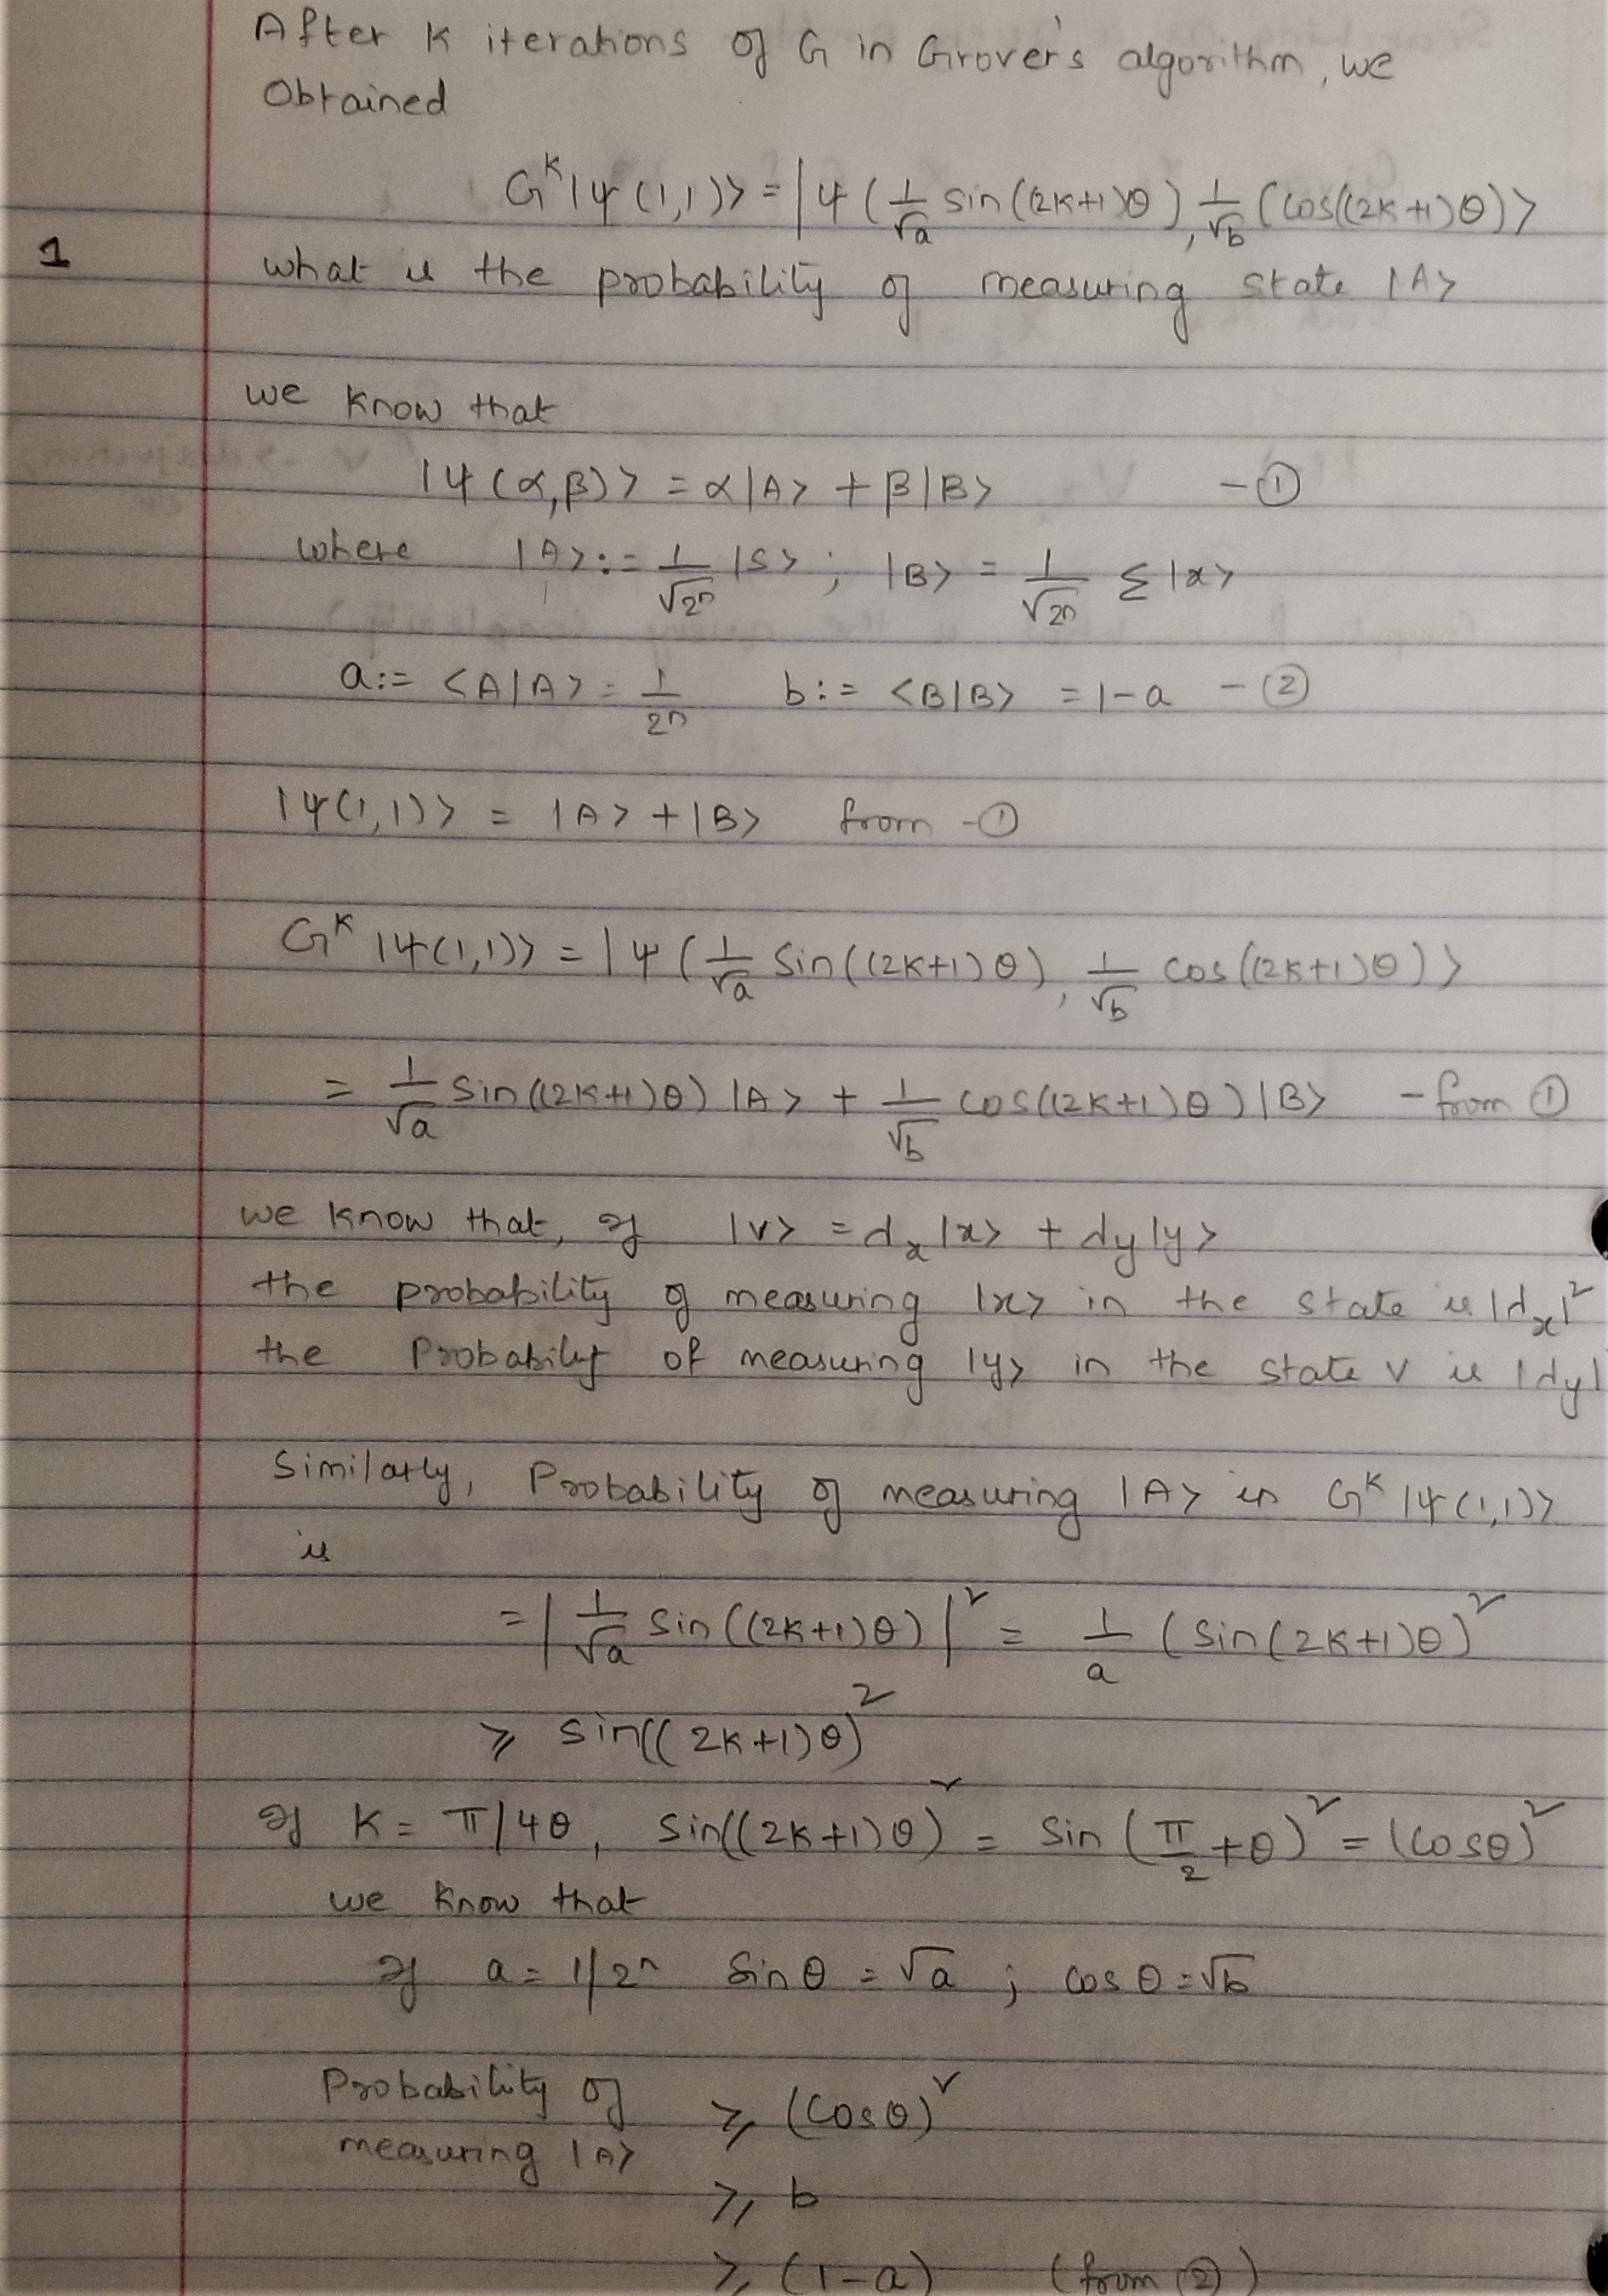
\includegraphics[width=18cm, height=23cm]{I22}

\newpage

{\bf 2.} \\
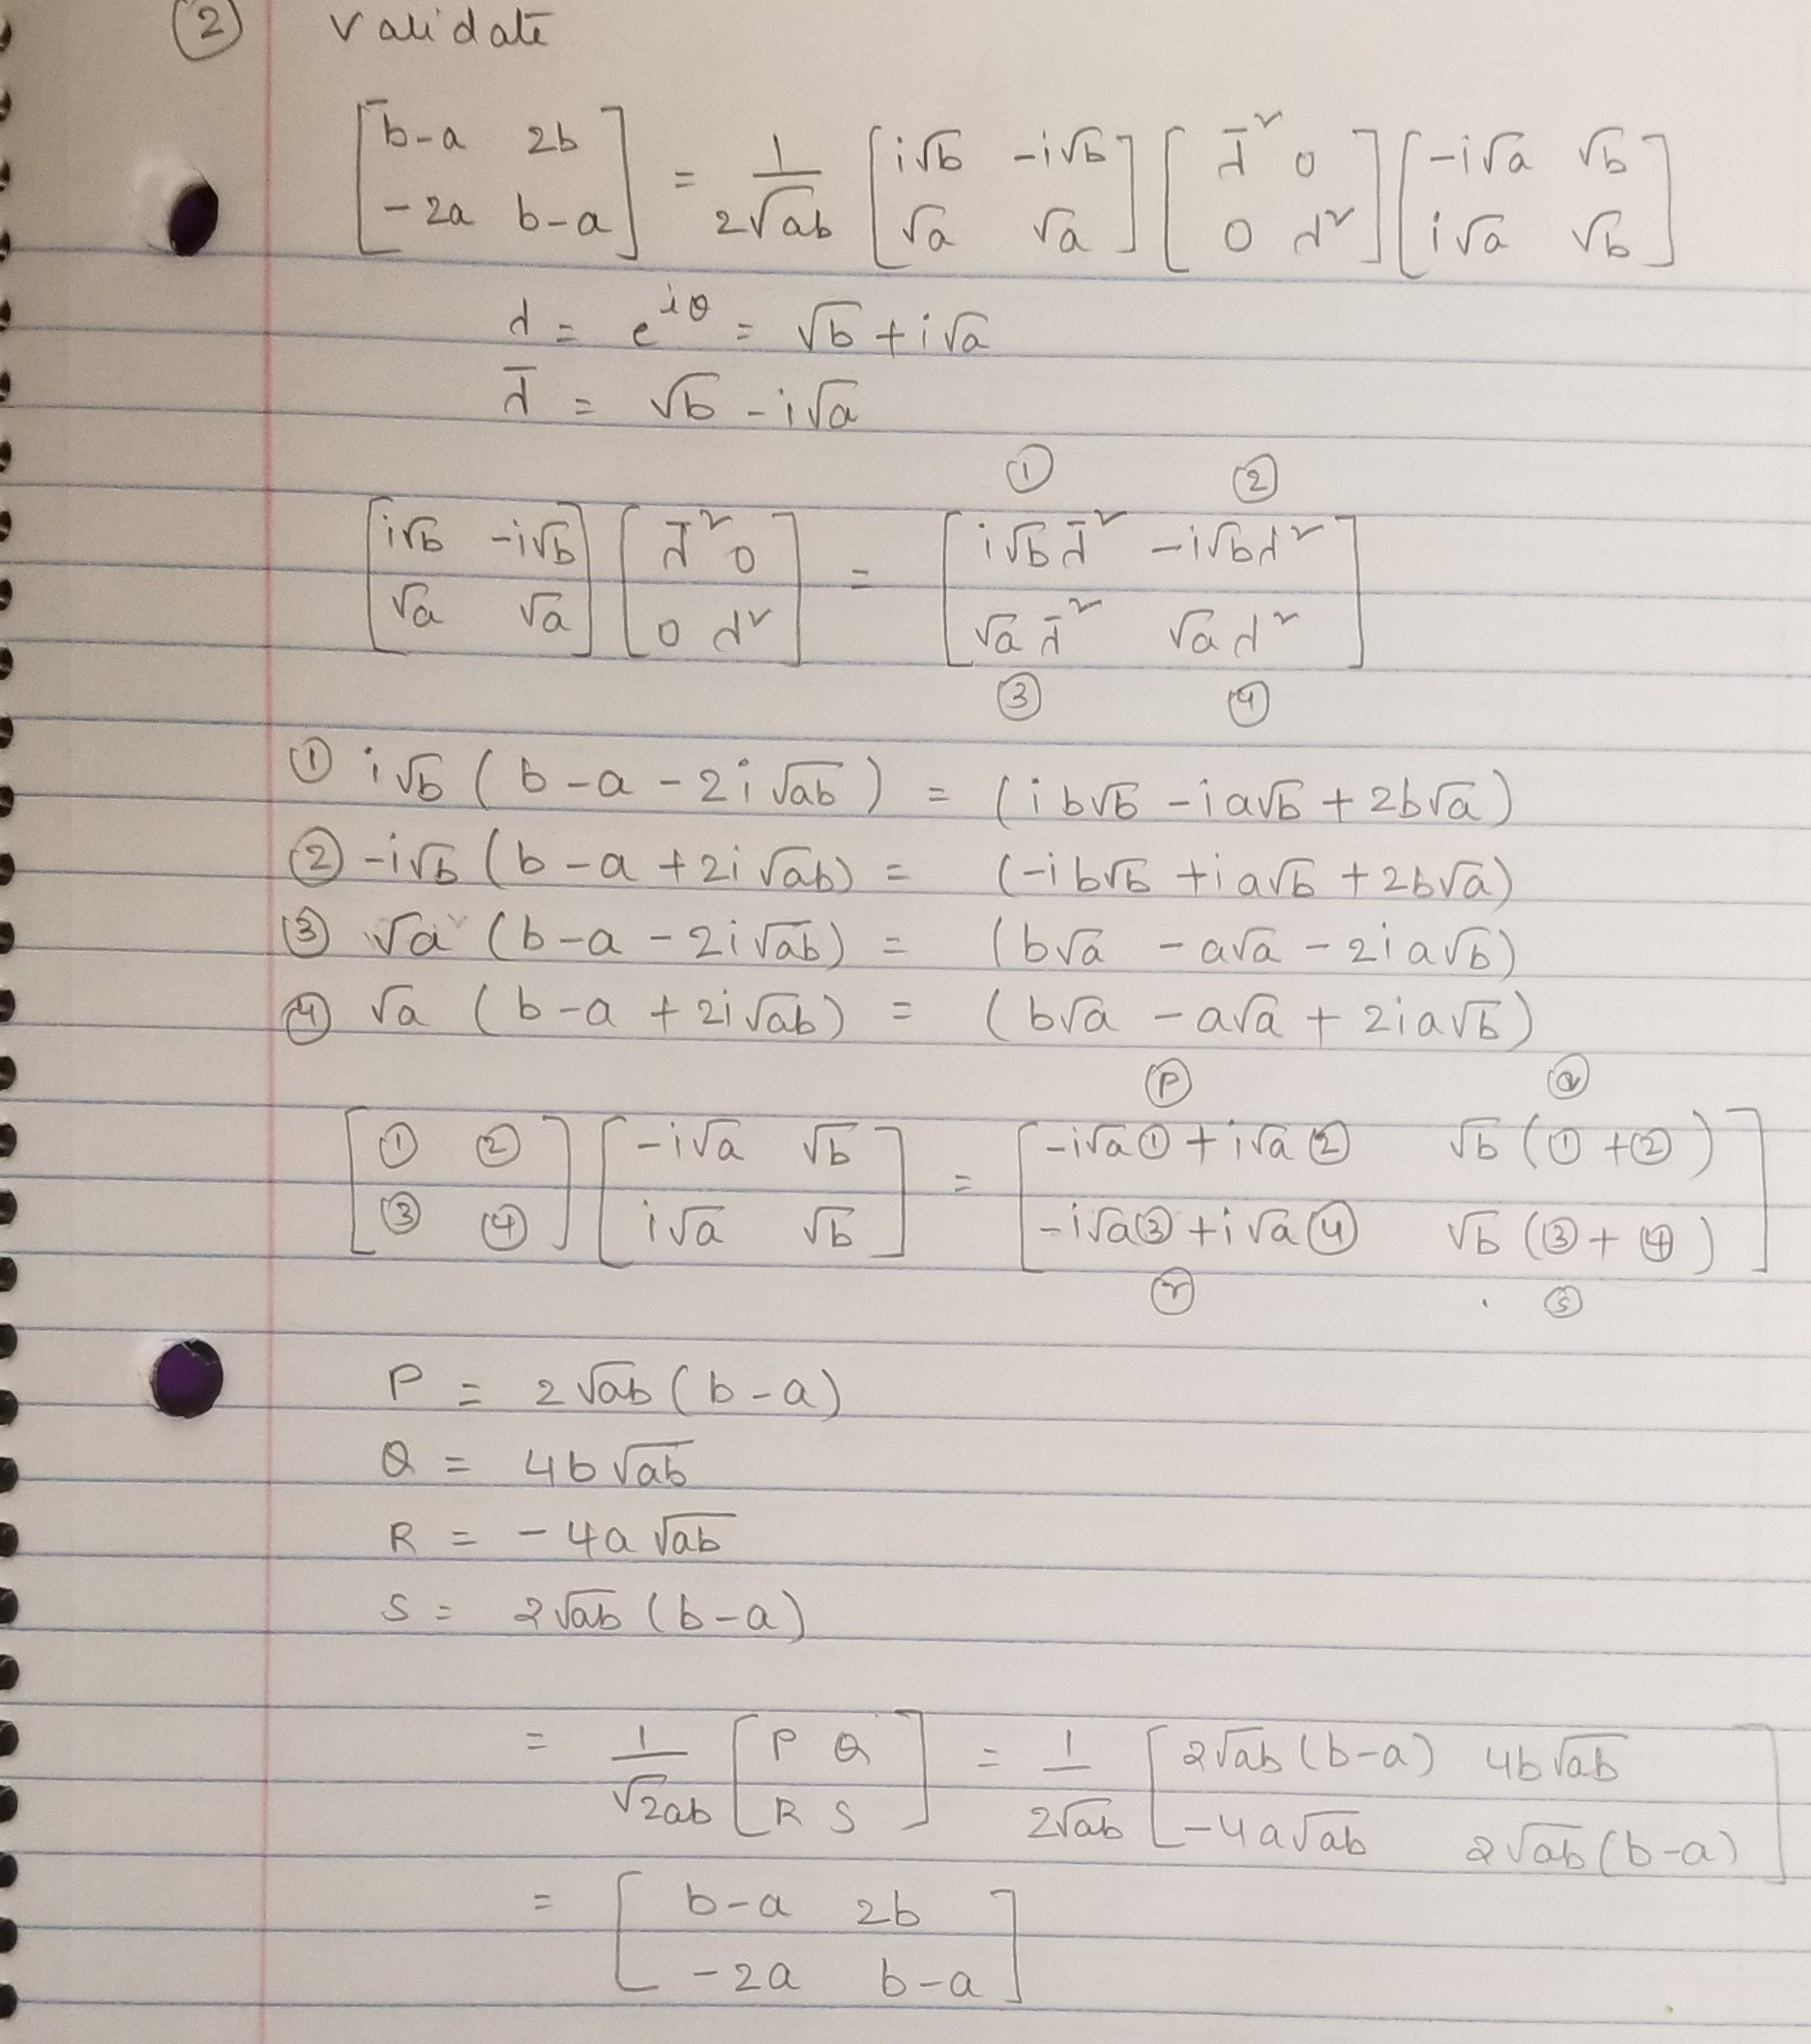
\includegraphics[width=18cm, height=23cm]{I11}

\end{document}